\chapter{\ifcpe บทนำ\else Introduction\fi}

\section{\ifcpe ที่มาของโครงงาน\else Project rationale\fi}
\label{sec:project_rationale}


การสอบปลายภาคหรือการทดสอบความรู้ในช่วงท้ายของการเรียนเป็นส่วนหนึ่งในการวัดระดับความรู้ที่นักศึกษาได้เรียนรู้ไปในวิชานั้น ๆ 
ซึ่งสามารถบ่งบอกถึงความเข้าใจ เอาใจใส่ของนักศึกษาคนนั้น ๆ ซึ่งปัจจัยที่มีผลต่อการสอบนั้นมีอยู่หลายปัจจัย 
ตัวอย่างเช่น ความตั้งใจ ความพยายาม ความเอาใจใส่กับรายวิชาของนักศึกษา แต่ก็ยังมีปัจจัยอีกหนึ่งปัจจัยที่มีผลต่อการสอบปลายภาคด้วย 
คือตารางสอบปลายภาคของนักศึกษา โดยตารางสอบนั้นอาจจะส่งผลกระทบต่อนักศึกษาหากทางมหาวิทยาลัยมีการจัดตารางสอบไม่ดีพอ 
ซึ่งในที่นี้จะกล่าวถึงการจัดตารางสอบของมหาวิทยาลัยเชียงใหม่ ซึ่งในแต่ละภาคการศึกษานั้นมีนักศึกษาที่เรียนมากกว่า 30000 คน
มีวิชาที่เปิดให้ลงทะเบียนมากกว่า 3000 วิชา มีคู่วิชาที่มีนักศึกษาลงทะเบียนพร้อมกันอย่างน้อย 1 คน มากกว่า 30000 คู่วิชา 
โดยตารางสอบนั้นจะเป็นตารางที่ถูกจัดไว้ก่อนการลงทะเบียนเรียนของนักศึกษา ในการลงทะเบียนเรียน นักศึกษาจะต้องพิจารณาเวลาสอบ และเลือกลงทะเบียนไม่ให้มีวิชาที่สอบตรงกัน 
มิฉะนั้นนักศึกษาจะต้องถอนวิชาใดวิชาหนึ่งที่เวลาสอบตรงกันออก หรือจะได้รับผลการประเมินขั้น F ในวิชาที่ไม่สามารถเข้าสอบปลายภาคได้


ทางมหาวิทยาลัยเชียงใหม่คาดหวังว่านักศึกษาจะเลือกลงทะเบียนเรียนวิชาต่าง ๆ โดยเลือกลงวิชาที่เวลาเรียนไม่ตรงกัน 
ดังนั้น ทางมหาวิทยาลัยจึงจัดตารางสอบของนักศึกษาให้กับวิชาที่มีตอนเดียวก่อน โดยจะอ้างอิงตามช่วงเวลาที่เรียน 
วิชาที่เรียนในวันและเวลาเดียวกันจะถูกจัดให้สอบในช่วงเวลาเดียวกัน (เรียกการจัดสอบแบบนี้ว่า Regular Exam ดังแสดงในรูปที่ \ref{fig:regular_exam}) 
%
\CIreply{ใส่ reference อ้างอิงรูปใน caption}
\begin{figure}
    \centering
    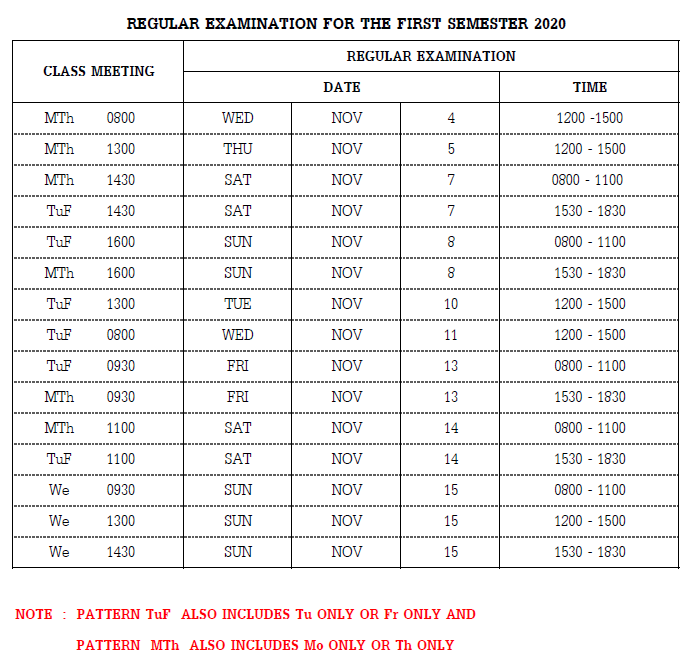
\includegraphics[width=\linewidth]{images/regular_exam.png}
    \caption[ตัวอย่างตารางสอบ regular exam ภาคการศึกษา 1/2563]{ตัวอย่างตารางสอบ regular exam ภาคการศึกษา 1/2563}
    \label{fig:regular_exam}
\end{figure}
%
ส่วนวิชาที่มีหลายตอน และอาจจะเปิดสอนหลายช่วงเวลา จะถูกจัดให้สอบในช่วงเวลาที่ไม่ตรงกับเวลาสอบของวิชาที่มีตอนเดียว  (เรียกการจัดสอบแบบนี้ว่า Special Exam ดังแสดงในรูปที่ \ref{fig:special_exam}) 
%
\CIreply{ใส่ reference อ้างอิงรูปใน caption}
\begin{figure}
    \centering
    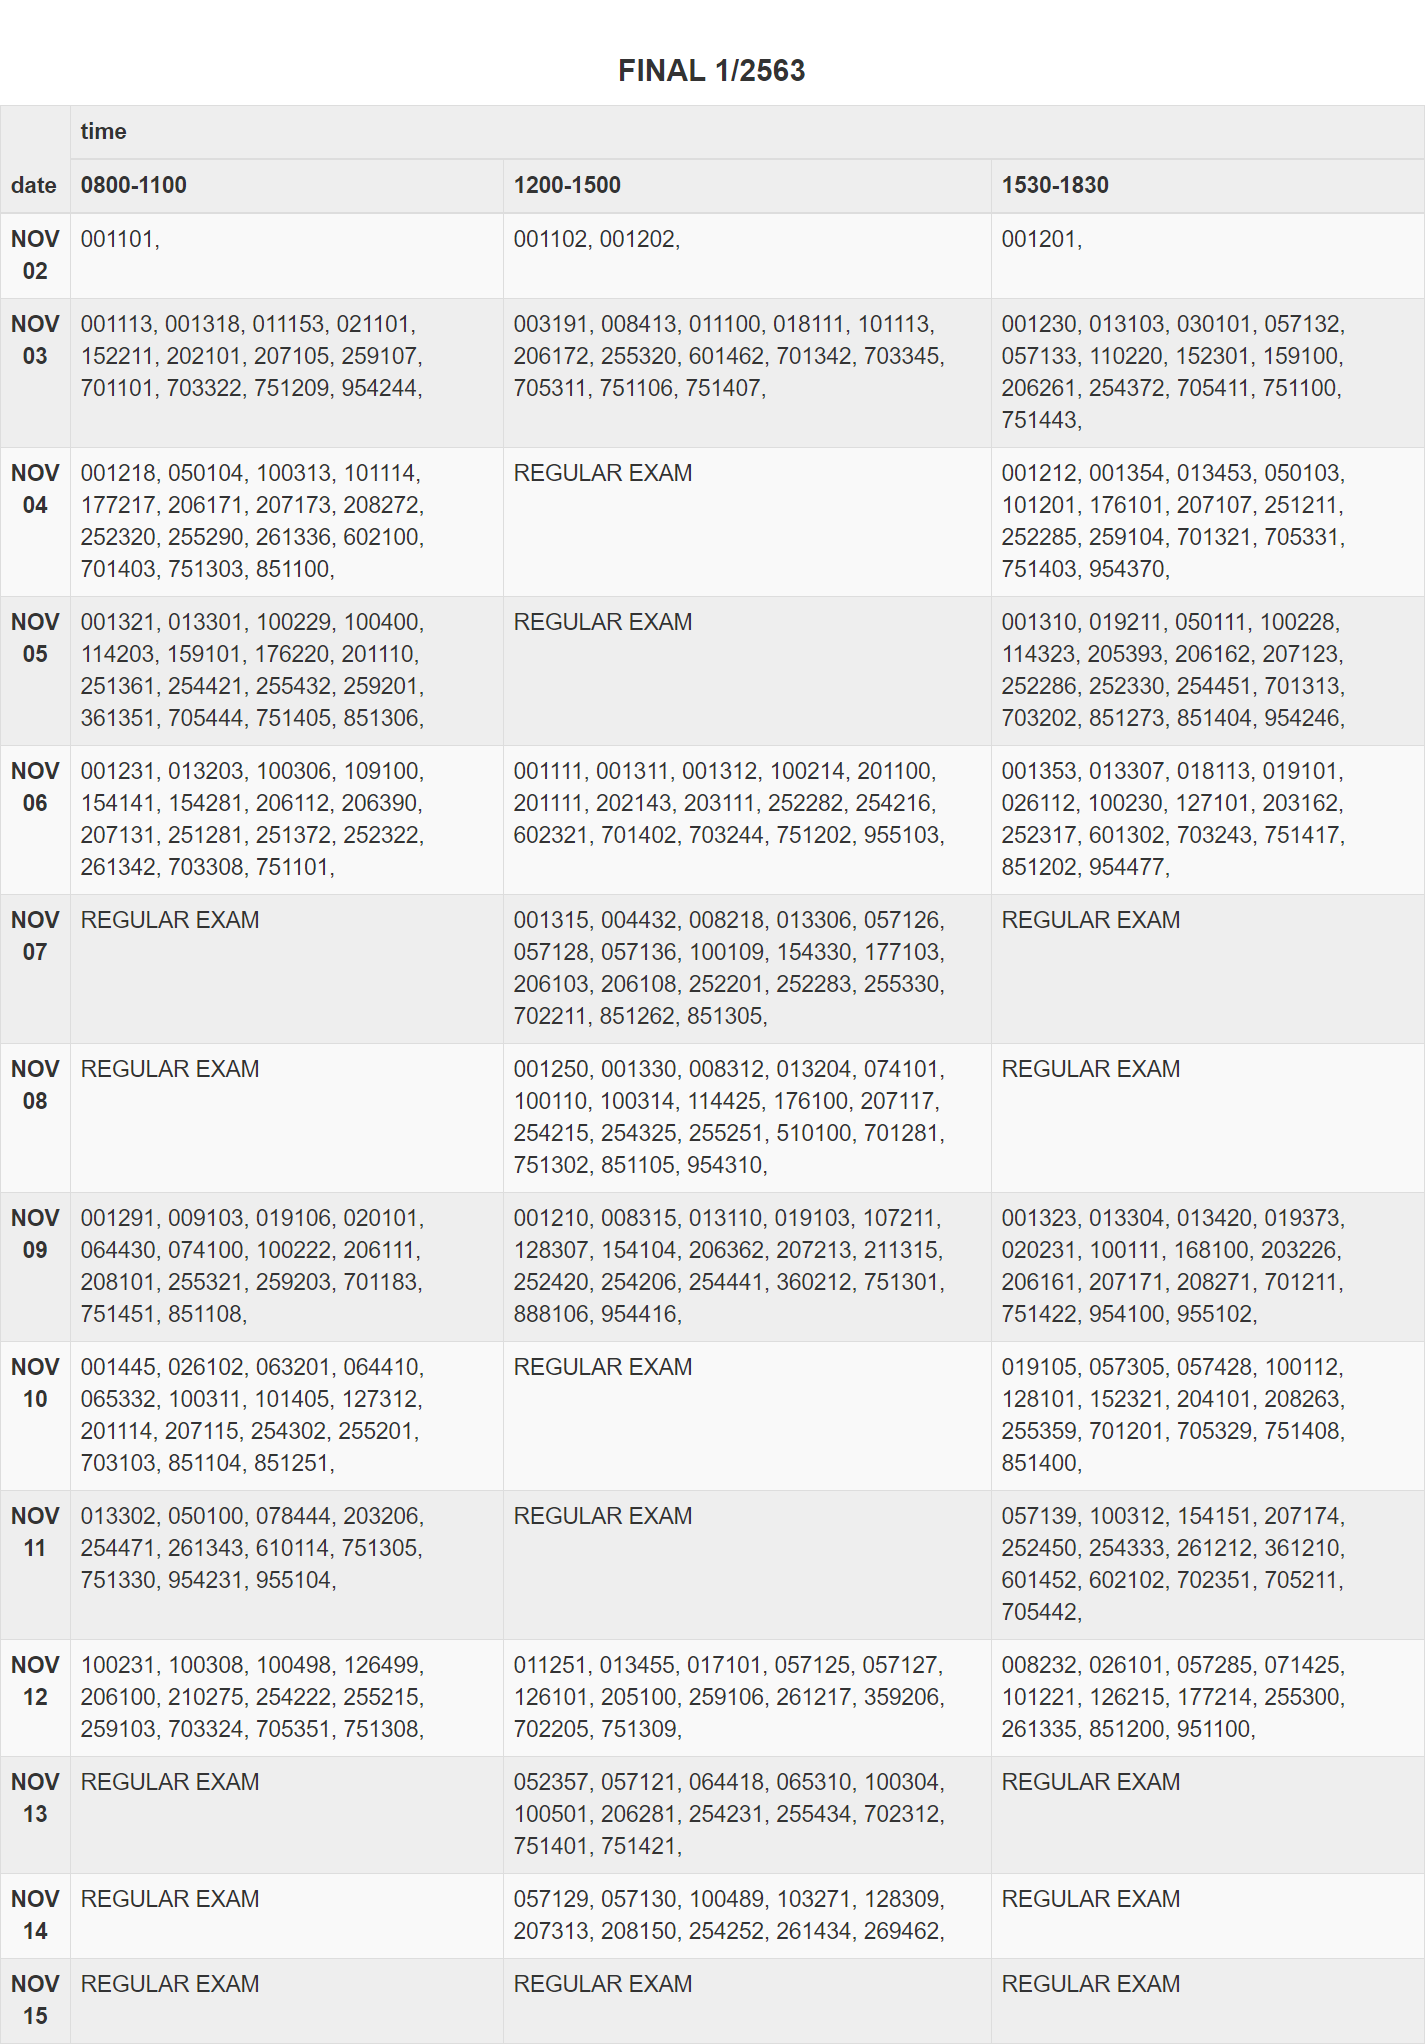
\includegraphics[width=\linewidth]{images/special_exam.png}
    \caption[ตัวอย่างตารางสอบ special exam ภาคการศึกษา 1/2563]{ตัวอย่างตารางสอบ special exam ภาคการศึกษา 1/2563}
    \label{fig:special_exam}     
\end{figure}
เพื่อให้นักศึกษาทั้งหมดที่ลงทะเบียนวิชาเดียวกัน แต่อาจจะคนละตอนกัน สามารถสอบในเวลาเดียวกันได้ เป็นการป้องกันข้อสอบรั่วไหลทางหนึ่ง 
ซึ่งการจัดตารางสอบในลักษณะดังกล่าวนั้นทําให้นักศึกษาไม่สามารถลงทะเบียนวิชาที่สนใจได้อย่างอิสระ เนื่องจากตารางสอบตรงกันหรือเวลาสอบของสองวิชาที่ต้องการลงทะเบียนนั้นติดกันมากเกินไป นอกจากนี้ การจัดตารางสอบด้วยวิธีนี้ ทำให้บางวิชานั้นถูกกําหนดวันสอบให้อยู่ในช่วงท้าย ๆ ของฤดูกาลสอบ 
ทําให้นักศึกษาบางคนมีวันเว้นว่างระหว่างการสอบหลายวันเพราะจําเป็นต้องอยู่รอทำการสอบในวิชาท้าย ๆ ซึ่งปัญหาดังที่กล่าวมานี้ก็อาจเกิดขึ้นกับมหาวิทยาลัยอื่น ๆ ที่มีวิธีการจัดการกับตารางสอบในรูปแบบที่คล้าย ๆ กันนี้เช่นกัน


แม้ว่างานวิจัยของ Ender {\"O}zcan~\cite{fes} จะได้สร้างโปรแกรมสำหรับจัดตารางสอบมาก่อน โดยมีการจัดตารางสอบแบ่งเป็นตารางสอบของวิชาภายในคณะและวิชาภายในภาควิชา 
แต่ก็ไม่สามารถใช้ได้กับวิชาเรียนของทางมหาวิทยาลัยเชียงใหม่ เนื่องจากมีวิชาศึกษาทั่วไป (General Education) ที่มีนักศึกษาจากต่างคณะสามารถลงทะเบียนเรียนร่วมกันได้
\CIreply{หากมีงานอื่นๆ ที่เกี่ยวข้อง เอามาใส่ตรงนี้ ใส่อย่างเดียวดูโดดเดี่ยวไปหน่อย}

จากปัญหาข้างต้น ทีมผู้พัฒนาคาดว่าการพัฒนาระบบจัดตารางสอบโดยใช้ข้อมูลลงทะเบียนของนักศึกษา หลังจากการลงทะเบียนเสร็จสิ้นแล้ว 
จะช่วยให้นักศึกษามีอิสระในการเลือกลงวิชาเรียนมากขึ้น ช่วยลดจำนวนนักศึกษาที่ต้องสอบสองวิชาติดกันในหนึ่งวันให้น้อยลง และลดวันเว้นว่างระหว่างช่วงเวลาสอบ
ซึ่งจะช่วยลดความเครียดส่วนหนึ่งในช่วงสอบของนักศึกษาได้

\section{\ifcpe วัตถุประสงค์ของโครงงาน\else Objectives\fi}
\label{sec:Objectives}
\begin{enumerate}
    \item เพื่อพัฒนาโปรแกรมสำหรับจัดตารางสอบปลายภาคในมหาวิทยาลัย จากข้อมูลการลงทะเบียนของนักศึกษา โดยตารางสอบที่ได้ต้องมีคุณสมบัติดังนี้
    \begin{itemize}
        \item ต้องไม่มีนักศึกษาคนใด ๆ ถูกกำหนดให้สอบสองวิชาในเวลาเดียวกัน
        \item จำนวนนักศึกษาที่มีสอบหลายวิชาติดกันในวันเดียว ลดลงจากตารางสอบดั้งเดิม
        \item จำนวนนักศึกษาที่มีช่วงวันที่เว้นจากการสอบวิชาก่อนหน้ามากกว่า 3 วัน ลดลงจากตารางสอบดั้งเดิม
        \item ในแต่ละช่วงเวลาที่จัดสอบ จำนวนนักศึกษาที่สอบจะต้องไม่เกินจำนวนที่นั่งสอบที่ทางมหาวิทยาลัยสามารถจัดให้ได้
    \end{itemize}
    \item เพื่อขจัดปัญหานักศึกษาไม่สามารถลงทะเบียนในรายวิชาที่ต้องการได้อย่างอิสระ เนื่องจากตารางสอบของรายวิชาที่ต้องการลงทะเบียนถูกจัดไว้ล่วงหน้าให้สอบในช่วงเวลาเดียวกัน
\end{enumerate}

\section{\ifcpe ขอบเขตของโครงงาน\else Project scope\fi}
เป้าหมายของโครงงานนี้ ต้องการพัฒนาโปรแกรมสำหรับจัดตารางสอบปลายภาคในระดับมหาวิทยาลัย
โดยโครงงานนี้จะพิจารณาความต้องการและข้อจำกัดต่าง ๆ ที่ใช้ในการจัดตารางสอบของมหาวิทยาลัยเชียงใหม่
และจะพิจารณาเฉพาะข้อจำกัดทางด้านเวลาเท่านั้น โดยมีขอบเขตของโครงงานดังนี้ 
\subsection{\ifcpe ขอบเขตด้านฮาร์ดแวร์\else Hardware scope\fi}
\begin{enumerate}
    \item ระบบที่จะพัฒนานั้นจะสามารถทำงานได้บนคอมพิวเตอร์ที่ใช้ระบบปฏิบัติการ Windows 7 / Windows 10 หรือระบบปฏิบัติการ Linux เท่านั้น
\end{enumerate}
\subsection{\ifcpe ขอบเขตด้านซอฟต์แวร์\else Software scope\fi}
\begin{enumerate}
    \item ระบบที่จะพัฒนานั้นจะสามารถทำงานได้หากติดตั้ง Python 3.7 ขึ้นไป เท่านั้น \TSNAreply{ไม่แน่ใจ ใส่ไว้ก่อน}
\end{enumerate}
\subsection{ตัวแปรที่นำมาพิจารณาในการจัดตารางสอบ}
\begin{enumerate}
    \item ระยะเวลาที่ใช้ในการจัดสอบปลายภาค คือ 2 สัปดาห์
    \item จำนวนช่วงเวลาที่จัดสอบในแต่ละวัน คือ 3 ช่วงเวลา ได้แก่ 8:00--11:00, 12:00--15:00, 
    และ 15:30--18:30
    \item จำนวนนักศึกษาที่ลงทะเบียนในแต่ละรายวิชา
    \item จำนวนที่นั่งสอบที่มหาวิทยาลัยสามารถจัดให้ได้ในตึกอาคารเรียนรวม
    \item จำนวนที่นั่งสอบในแต่ละห้องสอบของแต่ละคณะ
    \item รายชื่อวิชาเรียนที่มีการจัดสอบปลายภาค
    \item ข้อมูลจากการลงทะเบียนล่วงหน้าและลงทะเบียนรอบปกติ
\end{enumerate}

\subsection{ตัวแปรที่ไม่นำมาพิจารณาในการจัดตารางสอบ}
\begin{enumerate}
    \item การจัดให้ห้องสอบให้กับแต่ละรายวิชา
    \item การจัดกรรมการคุมสอบให้กับแต่ละรายวิชา
    \item เวลาเรียนของแต่ละรายวิชา (ซึ่งมีบทบาทสำคัญในการจัดตารางสอบแบบเดิม)
    \item การเลือกช่วงเวลาสอบให้กับแต่ละรายวิชาโดยอาจารย์ผู้สอนวิชานั้น ๆ
    \item ข้อมูลจากการลงทะเบียนเพิ่มเติมหลังกำหนด
\end{enumerate}

\section{\ifcpe ประโยชน์ที่ได้รับ\else Expected outcomes\fi}
\begin{enumerate}
    \item นักศึกษาสามารถเลือกลงทะเบียนวิชาที่ต้องการได้อย่างอิสระ โดยไม่ต้องกังวลว่าวิชาเหล่านั้นจะถูกจัดให้สอบในช่วงเวลาเดียวกัน
    \item ช่วยให้ตารางสอบของนักศึกษาคนใด ๆ มีจำนวนรายวิชาที่ต้องสอบในแต่ละวันน้อยลง
    \item ช่วยลดวันเว้นว่างระหว่างช่วงเวลาสอบของนักศึกษาให้น้อยลง
    \item ช่วยให้จำนวนนักศึกษาที่ต้องสอบในแต่ช่วงเวลาสอบไม่มากจนเกินไป
\end{enumerate}
\CIreply{อาจจะพูดถึงเรื่องที่นั่งสอบ ที่ไม่ overload ใน regular slot สำหรับ เวลาเรียนที่ prime time}

\section{\ifcpe เทคโนโลยีและเครื่องมือที่ใช้\else Technology and tools\fi}

% \subsection{\ifcpe เทคโนโลยีด้านฮาร์ดแวร์\else Hardware technology\fi}
% \begin{enumerate}

% \end{enumerate}
\subsection{\ifcpe เทคโนโลยีด้านซอฟต์แวร์\else Software technology\fi}
\begin{enumerate}
    \item Visual Studio Code ใช้สำหรับการเขียนโปรแกรมสำหรับจัดตารางสอบ และเขียนเว็บแอปพลิเคชันสำหรับให้นักศึกษาใช้ประเมินความพึงพอใจของตารางสอบ
    \item Python เป็นภาษาหลักที่ใช้ในการพัฒนาโปรแกรมสำหรับจัดตารางสอบในโครงงานนี้
    \item Node.js ใช้เป็น Back-end เพื่อเปิดเซิร์ฟเวอร์ของเว็บแอปพลิเคชันสำหรับให้นักศึกษาใช้ประเมินความพึงพอใจของตารางสอบ
    \item Vue.js ใช้สำหรับช่วยในการแสดงผลหน้าเว็บและเชื่อมต่อข้อมูลกับ Back-end สำหรับเว็บแอปพลิเคชันสำหรับให้นักศึกษาใช้ประเมินความพึงพอใจของตารางสอบ
    \item MongoDB ใช้เป็นฐานข้อมูลสำหรับเก็บตารางสอบของนักศึกษาแต่ละคนเพื่อนำมาแสดงบนเว็บแอปพลิเคชันสำหรับให้นักศึกษาใช้ประเมินความพึงพอใจของตารางสอบ
\end{enumerate}
\CIreply{อธิบายเพิ่มเติมคร่าวๆ ว่าแต่ละอย่างใช้เพื่ออะไร}

\section{\ifcpe แผนการดำเนินงาน\else Project plan\fi}
ในแผนการดำเนินงานของโครงงานนี้ ในส่วนของ Literature review จะเป็นการทบทวนงานเขียนและผลงานที่มีความเกี่ยวข้องกับการจัดตารางสอบ
ทั้งทฤษฎี อัลกอริทึมและระบบ ที่เคยมีการสร้างขึ้นมาก่อนแล้วเป็นต้น ในส่วนของการเก็บข้อมูลความคิดเห็นนักศึกษาครั้งที่ 1 นั้น
จะเป็นการเก็บข้อมูลความคิดเห็นของนักศึกษาเกี่ยวกับ ข้อดี ข้อเสีย และความพึงพอใจในตารางสอบของตนเอง รวมถึงปัญหาเกี่ยวกับตารางสอบปลายภาคที่นักศึกษาเคยพบหรือได้รับผลกระทบจากปัญหานั้นโดยตรง
เพื่อนำข้อมูลมาออกแบบอัลกอริทึม และ penalty model ในการจัดตารางสอบให้ตรงตามความต้องการของนักศึกษา


การออกแบบอัลกอริทึมและ penalty model เวอร์ชัน 1 นั้นเป็นการทดลองออกแบบอัลกอริทึมให้สามารถจัดตารางสอบได้
โดยใช้ penalty model ที่เป็นผลจากการเก็บข้อมูลความคิดเห็นนักศึกษาครั้งที่ 1 
ซึ่งจะแตกต่างจากการออกแบบอัลกอริทึมและ penalty model เวอร์ชัน 2
ตรงที่ในเวอร์ชัน 2 ได้มีการปรับเปลี่ยนอัลกอริทึมให้ทำงานได้ถูกต้องและเร็วขึ้น และได้เพิ่มข้อจำกัดเกี่ยวกับความจุที่นั่งสอบในการจัดสอบในแต่ละช่วงเวลาเข้าไปใน penalty model ด้วย


สำหรับการเก็บข้อมูลความพึงพอใจและความคิดเห็นของนักศึกษาครั้งที่ 2 เพื่อใช้ในการประเมินผลอัลกอริทึม นั้นจะเป็นการให้นักศึกษาทำ A/B testing 
ผ่านเว็บแอปพลิเคชันซึ่งนักศึกษาจะต้อง
ล็อกอินผ่าน OAuth ด้วย CMU Account แล้วแสดงข้อมูลตารางสอบของตนเอง ภาคการศึกษาละ 2 แบบ เปรียบเทียบกัน
โดยแบบหนึ่งจะเป็นตารางสอบที่กำหนดโดยสำนักทะเบียนและประมวลผล มหาวิทยาลัยเชียงใหม่ 
อีกแบบหนึ่งจะเป็นตารางสอบที่จัดโดยอัลกอริทึมที่ได้ออกแบบไป โดยนักศึกษาจะไม่ทราบว่าตารางสอบที่เห็นแต่ละด้านนั้นเป็นแบบใด และให้นักศึกษาเลือกตารางสอบที่ชอบพร้อมทั้งระบุเหตุผลที่ชอบตารางสอบแบบที่เลือก
และให้นักศึกษาสามารถแสดงความคิดเห็นอื่น ๆ เกี่ยวกับตารางสอบได้ด้วยเช่นกัน

\begin{plan}{7}{2020}{3}{2021}
    \planitem{7}{2020}{10}{2020}{Literature review}
    \planitem{9}{2020}{10}{2020}{เก็บข้อมูลความคิดเห็นนักศึกษาครั้งที่ 1}
    \planitem{10}{2020}{10}{2020}{เขียนโครงร่างรายงาน}
    \planitem{11}{2020}{12}{2020}{เก็บข้อมูลรายวิชาที่มีการจัดสอบ}
    \planitem{11}{2020}{12}{2020}{ออกแบบอัลกอริทึมและ penalty model เวอร์ชัน 1}
    \planitem{12}{2020}{12}{2020}{ทดสอบและประเมินผลอัลกอริทึม เวอร์ชัน 1 ด้วย penalty model}
    \planitem{12}{2020}{1}{2021}{เก็บข้อมูลความจุที่นั่งสอบของแต่ละคณะและอาคารส่วนกลาง}
    \planitem{12}{2020}{1}{2021}{ออกแบบอัลกอริทึมและ penalty model เวอร์ชัน 2}
    \planitem{1}{2021}{2}{2021}{ทดสอบและประเมินผลอัลกอริทึม เวอร์ชัน 2 ด้วย penalty model}
    \planitem{2}{2021}{3}{2021}{ประเมินผลระบบโดยการเก็บข้อมูลความพึงพอใจและความคิดเห็นของนักศึกษา}
    \planitem{2}{2021}{3}{2021}{สรุปผลการพัฒนาโปรแกรม}
    \planitem{3}{2021}{3}{2021}{เขียนรายงานผลการพัฒนาโปรแกรม}
\end{plan}

\CIreply{ความคิดเห็นแต่ละครั้ง ต่างกันอย่างไร}
\CIreply{อธิบายความแตกต่างของ versions 1 \& 2}
\CIreply{อาจจะเขียนเป็นร้อยแก้วก่อนขึ้นตาราง}
\TSNAreply{มัน Tab ตารางตรงนี้เข้าไป แก้ไม่เป็นครับ}

\section{\ifcpe บทบาทและความรับผิดชอบ\else Roles and responsibilities\fi}
\begin{itemize}
    \item นายกฤษฏิ์ อุปนันท์: รับผิดชอบหน้าที่ในการเก็บรวบรวมและสรุปผลความคิดเห็นและความต้องการของนักศึกษา
    จากแบบสำรวจเพื่อนำมาใช้ในการจัดลำดับความสำคัญของตัวชี้วัดที่ใช้ในการประเมินระบบ ออกแบบ penalty model สำหรับใช้ในการประเมินระบบ 
    ออกแบบหน้าเว็บและพัฒนาส่วน Front-end และการแสดงผลของเว็บแอปพลิเคชันสำหรับใช้เก็บข้อมูลความพึงพอใจและความคิดเห็นของนักศึกษา เพื่อใช้ในการประเมินระบบ
    \item นายธนวงศ์ เสนีวงศ์ ณ อยุธยา: รับผิดชอบหน้าที่ในการศึกษาทฤษฎีที่เกี่ยวข้องและอัลกอริทึมที่จำเป็นต้องใช้ในการพัฒนาระบบจัดตารางสอบ 
    ออกแบบอัลกอริทึมและพัฒนาระบบจัดตารางสอบและและโปรแกรมเพื่อประเมินระบบตาม penalty model 
    จัดการทำความสะอาดข้อมูล (data cleansing) สำหรับข้อมูลรายวิชาที่มีการจัดสอบ และข้อมูลความจุที่นั่งสอบของแต่ละคณะและอาคารส่วนกลาง
    ออกแบบฐานข้อมูลและพัฒนาส่วน Back-end ของเว็บแอปพลิเคชันสำหรับใช้เก็บข้อมูลความพึงพอใจและความคิดเห็นของนักศึกษา
    จัดการทำความสะอาดข้อมูลและสรุปผล ข้อมูลความพึงพอใจและความคิดเห็นของนักศึกษา เพื่อใช้ในการประเมินระบบ
\end{itemize}

\section{\ifcpe%
ผลกระทบด้านสังคม สุขภาพ ความปลอดภัย กฎหมาย และวัฒนธรรม
\else%
Impacts of this project on society, health, safety, legal, and cultural issues
\fi}

% ผลกระทบทางด้านสังคม: 
ระบบที่เป็นผลลัพธ์ของโครงงานนี้จะสามารถใช้เป็นทางเลือกในการจัดการตารางสอบปลายภาคในระดับมหาวิทยาลัยได้
ซึ่งตัวระบบได้เปลี่ยนแปลงลำดับขั้นตอนการทำงานของระบบลงทะเบียนด้วย โดยขั้นตอนที่เปลี่ยนแปลงไปนี้จะช่วยให้นักศึกษาสามารถเลือกลงทะเบียนเรียนวิชาที่ตนเองต้องการได้อย่างอิสระ 
โดยไม่ต้องกังวลว่าวิชาเหล่านั้นจะถูกจัดให้สอบในช่วงเวลาเดียวกัน เหมือนอย่างระบบเดิมที่ทางมหาวิทยาลัยเชียงใหม่ใช้อยู่ในปัจจุบัน
อีกทั้งตารางสอบปลายภาคที่ได้จากระบบนี้นั้นยังคำนึงถึงความสมดุลของตารางสอบของนักศึกษาโดยรวม ซึ่งจะช่วยให้นักศึกษาแต่ละคนมีตารางสอบที่เหมาะสมมากกว่าระบบเดิมที่ใช้จัดตารางสอบ
ทั้งการที่ไม่มีวิชาที่ถูกจัดให้สอบในช่วงเวลาเดียวกัน มีวิชาที่สอบติดกันน้อยลง ทำให้นักศึกษามีเวลาทบทวนวิชาที่ต้องสอบต่อไปมากขึ้น อีกทั้งยังพยายามจัดสอบให้มีเวลาเว้นว่างระหว่างวันสอบน้อยลง
ทำให้นักศึกษาสอบเสร็จได้เร็วขึ้น ซึ่งตารางสอบที่สมดุลขึ้นนี้อาจจะช่วยลดความเครียดความกดดันและภาระทางจิตใจของนักศึกษาในช่วงสอบให้ลดน้อยลงได้ ทำให้นักศึกษามีกำลังใจในการสอบ และรู้สึกว่าการสอบนั้นเหนื่อยน้อยลง
ซึ่งที่กล่าวมาทั้งหมดนี้จะเป็นตัวช่วยให้การวัดผลประเมินผลด้วยการสอบนั้นให้ผลที่ดีและแม่นยำมากขึ้น


ระบบที่ได้นี้หากนำไปพัฒนาต่อ เช่นพัฒนาให้ช่วยจัดห้องสอบให้แต่ละวิชาด้วย อาจจะช่วยให้การทำงานของบุคคลากรของมหาวิทยาลัยมีความสะดวกสบายมากขึ้น 
เพราะจากการที่ได้ไปสำรวจข้อมูลจากแต่ละคณะในหมาวิทยาลัย ยังมีหลายคณะที่คณาจารย์หรือบุคคลากรยังใช้วิธีจัดห้องสอบด้วยตัวเองอยู่ 
ซึ่งหากมีระบบที่จะทำงานให้อัตโนมัติก็จะช่วยช่วยลดภาระการจัดห้องสอบของบุคคลากรได้ และอาจจะสามารถประยุกต์ใช้ระบบนี้กับการสอบรูปแบบอื่น ๆ หรือใช้ในมหาวิทยาลัยอื่น ที่มีปัญหาเกี่ยวกับตารางสอบคล้าย ๆ กันแบบนี้ได้ด้วย
